\documentclass[12pt]{article}
\usepackage{graphicx}
\usepackage{hyperref}
\begin{document}
\author{\href{http://freecol.sourceforge.net/index.php?section=8}
  {The FreeCol Team}}
\title{FreeCol Documentation\\User Guide for Version v0.5.1}
\maketitle{}


\hypertarget{Introduction}{\section{Introduction}}

Welcome to FreeCol! If you're interested in development of this
program, please see the \href{http://freecol.sourceforge.net}{FreeCol
web site}. This is a draft version of the user's guide. You can find
the latest version at the
\href{http://freecol.sourceforge.net}{FreeCol homepage}.

%% \hypertarget{History}{\section{History}}
%% \label{history}
%% This section gives details about the history of this user guide.
%% \begin{itemize}
%% \item v0.2.0: add the �About� section and disband shortcut.
%% \item v0.1.2: corrections from Bryce Harrington and copyright notice.
%% \item v0.1.1: Main screen's, Colony panel's and Europe panel's images
%%   were added.
%% \item v0.1: Creation of the user guide! The guide contains the
%%   following sections: �Introduction�, �History�, �Installation� and
%%   �Interface�.
%% \end{itemize}



\hypertarget{About}{\section{About}}

\hypertarget{About FreeCol}{\subsection{About FreeCol}}

The FreeCol team aims to create an Open Source version of
Colonization (released under the
\href{http://www.gnu.org/licenses/gpl.html}{GPL}). At
first we'll try to make an exact clone of Colonization. The visuals
will be brought up to date with more recent standards but will remain
clean, simple and functional. Certain new 'features' will be
implemented but the gameplay and the rules will be exactly the same as
the original game. Examples of modern features are: an isometric map
and multiplayer support.

This clone will be developed incrementally and result in
\textbf{FreeCol 1.0.0 which will be an almost exact Colonization
clone}. Incremental development basically means that we'll add
features one at a time. This allows us to have a running program at
all times and also to release an unfinished but working game once in a
while.

Once FreeCol 1.0.0 is finished we'll start working towards FreeCol
2.0.0. \textbf{FreeCol 2 will go beyond the original Colonization} and
will have many new features, it will be an implementation of our (and
our users') image of what Colonization 2 would have been.

\hypertarget{The Original Colonization}{\subsection{The Original Colonization}}

The original Colonization was released in 1994 by Microprose.
\textbf{Colonization is heavily based on Civilization} which is
generally considered to be the best turn-based strategy game for the
PC in the history of mankind.

In Civilization the object of the game was to build a nation that
could stand the test of times and that could also do one of the
following: conquer the world or be the first to launch a
spaceship. In Colonization things are bit different...

A Colonization game starts in 1492 and \textbf{the object of the game
is to colonize America}. You begin the game with one vessel and two
colonists.

As in Civilization you need to build a powerful nation, but
fortunately in the early part of the game \textbf{you'll be able to
send ships back to Europe} in order to sell the goods you've produced
or to bring back some colonists. \textbf{Getting colonists into the
new world is a very important aspect of the game} as one game turn
takes one year and later on even one season and as a result colonies
don't grow as rapidly as they do in Civilization. You can pay
colonists to come to the new world or you can show off with the
religious freedom of your people in which case they will hop on your
vessels for no money at all.

Another important aspect is \textbf{trade: the source of all income}
(apart from Inca and Aztec gold). In a land filled with precious
resources it is important to \textbf{build your colonies at the right
location} and to place crafstmen where they belong. This is not only
to have an income but also to be able to \textbf{live off the land}
when you can no longer count on the support of Europe.

Through all this you'll have to decide whether or not you want to
\textbf{live next to the native americans} peacefully. They can teach
your colonists new skills that cannot be tought anywhere else and they
will offer you goods in case you choose to treat them as your
friends. On the other hand, their villages can be attacked and their
valuable goods can be taken from them and sold in Europe.

\textbf{Other European forces are also busy occupying their piece of
the new world}. Should their borders go too far then take over some
of their colonies by force because they wouldn't hesitate to do the
same thing to you.

The object of Colonization is to \textbf{declare your independence and
survive an attack of the King's forces}. Before declaring your
independence \textbf{you need to have the majority of the people
behind you}. This can be done by \textbf{promoting free speech} and by
providing a strong governmental system.

\hypertarget{Installation}{\section{Installation}}

To compile FreeCol you'll need Java and the Ant program. Ant can be
found at \href{Ant homepage}{http://ant.apache.org/}.

When these are installed, go to the root directory of FreeCol and type
\verb$ant$ to build a JAR file containing the game. The game is
started using the command \verb$java -jar FreeCol.jar$.  If something
goes wrong, send a bug report at the
\href{http://sourceforge.net/projects/freecol}{SourceForge page of
FreeCol}.

\hypertarget{Interface}{\section{Interface}}

This section will provide information about the keyboard shortcuts and
the different actions that can be used in the game.

\hypertarget{The main screen}{\subsection{The main screen}}

The figure \ref{main_screen_fig} represents the main screen.
\begin{figure}
  \begin{center}
    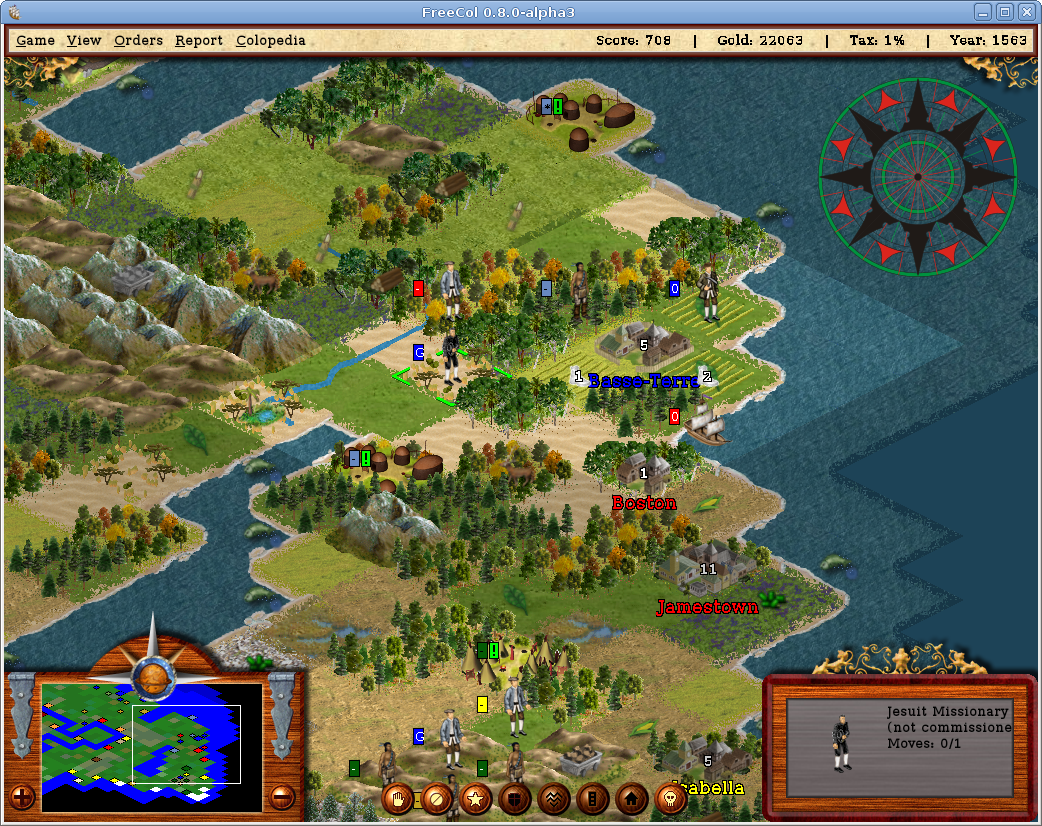
\includegraphics[scale=0.35]{images/main_screen.png}
    \caption{The main screen.\label{main_screen_fig}}
  \end{center}
\end{figure}

The units, colonies, and so forth can be seen on the main screen. You
can change the currently selected unit by clicking on any other
unit. You can move the currently selected unit using the numeric
keypad. If you select a unit with the left mouse button and drag the
mouse, the main screen will display the best path from the unit's
current position to the tile the mouse is hovering over. 

The tiles the path consists of will be marked with boots if the unit
is on foot, horseshoes if the unit is mounted, or sextants if the unit
is a naval unit. These symbols will also indicate whether the tiles
can be reached during this turn or not. Once you release the mouse
button, the selected unit will begin to follow this path. It will
awake once it has arrived at its destination or if it can no longer
follow the path (if an enemy unit is in the way, for instance).

If you right click on a tile containing neither units nor settlements,
a popup window will show you some information about the goods that can
be produced on this tile (unless the tile has not yet been explored,
in which case nothing will happen). If the tile contains units or
settlements, you will be presented with a menu from which you can
select the units or the settlement present, or the tile information.

The following shortcuts are also available:
\begin{itemize}
\item\verb$b$: build a colony.
\item\verb$c$: center on the currently selected unit.
\item\verb$d$: disband the active unit.
\item\verb$e$: show the Europe panel.
\item\verb$f$: fortify.
\item\verb$g$: goto selected destination.
\item\verb$p$: plow the current tile.
\item\verb$r$: build a road on the current tile.
\item\verb$s$: sentry (not implemented).
\item\verb$w$: wait.
\item\verb$space$: skip for this turn.
\item\verb$enter$: end the turn.
\item\verb$plus$ or \verb$equals$: zoom in.
\item\verb$minus$ or \verb$underscore$: zoom out.
\item\verb$ctrl-d$: display tile names.
\item\verb$ctrl-g$: display grid.
\item\verb$ctrl-m$: show/hide the map controls.
\item\verb$ctrl-n$: new game.
\item\verb$ctrl-o$: open a game.
\item\verb$ctrl-q$: quit the game.
\item\verb$ctrl-r$: reconnect.
\item\verb$ctrl-s$: save a game.
\item\verb$ctrl-t$: show the chat panel.
\end{itemize}

\hypertarget{The Europe panel}{\subsection{The Europe panel}}

The figure \ref{europe_panel_fig} represents the Europe panel.
\begin{figure}
  \begin{center}
    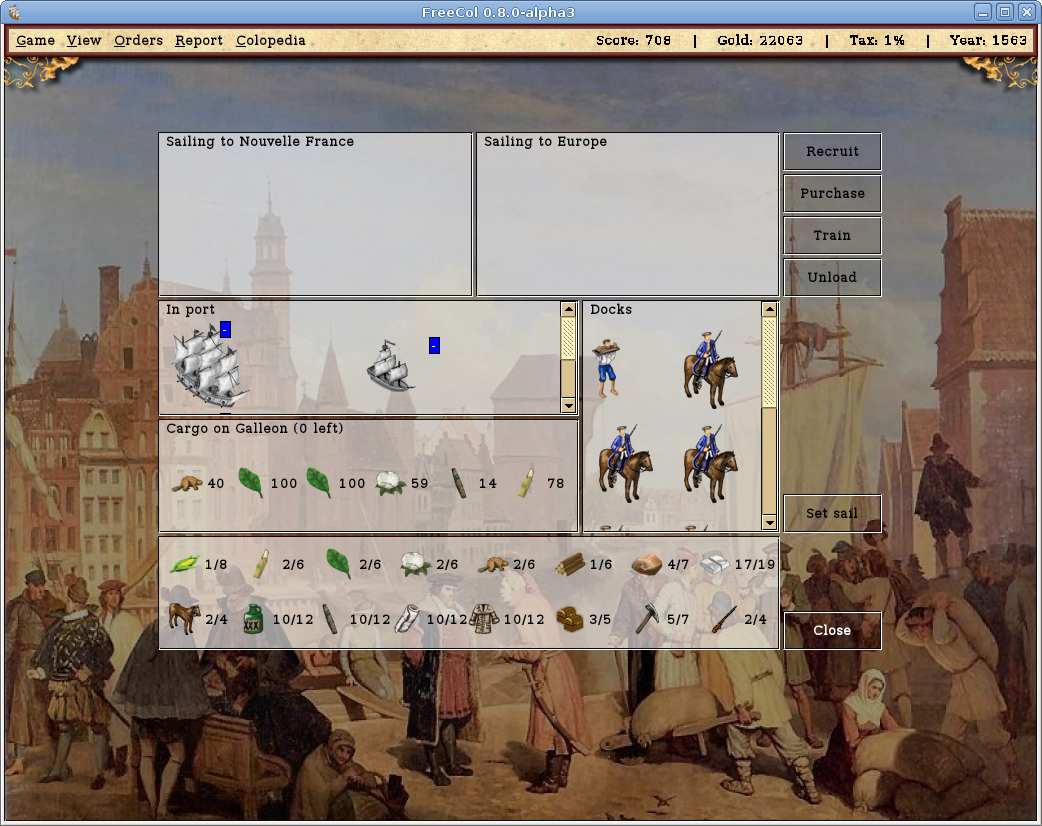
\includegraphics[scale=0.35]{images/europe_panel.png}
    \caption{The Europe Panel.\label{europe_panel_fig}}
  \end{center}
\end{figure}

In this panel, you can control the ships embarked for America or Europe,
and the ships currently stationed in Europe. You can also buy goods,
recruit, purchase and train units. Units recruited, purchased or trained
are in the �Docks� area in the Europe panel.

If a ship has set sail for Europe or America, you can change its
direction by dragging it from the �Going to America� box to the �Going
to Europe� box (or vice versa).

Ships that are docked at the European port can also do the following:
\begin{itemize}
\item Embark/Disembark units: drag and drop between the �Docks�
  and �Cargo� sections of the Europe panel.
\item Sell/Buy goods: drag and drop between the �Cargo� panel and the
  �Market� panel. If you want to sell only a part of your cargo, or
  want to buy less than 100 units of goods, press the shift key while
  dragging. This will allow you to specify how many units you wish to
  transfer. If any of the goods are displayed in grey, this means they
  are being boycotted by the Crown because you refused a tax
  raise. You must pay your tax arrears before you can trade these
  goods. You can do this by dragging the goods as usual, in which case
  you will be given the chance to pay your tax arrears (provided you
  have enough money).
\item Arm/Mount/Equip with tools/Dress as missionaries a unit: 
  right click on the unit.
\item Move your ship to the �Going to America� section of the Europe
  panel.
\end{itemize}

\hypertarget{The Colony panel}{\subsection{The Colony panel}}

The figure \ref{colony_panel_fig} represents the Colony panel.
\begin{figure}
  \begin{center}
    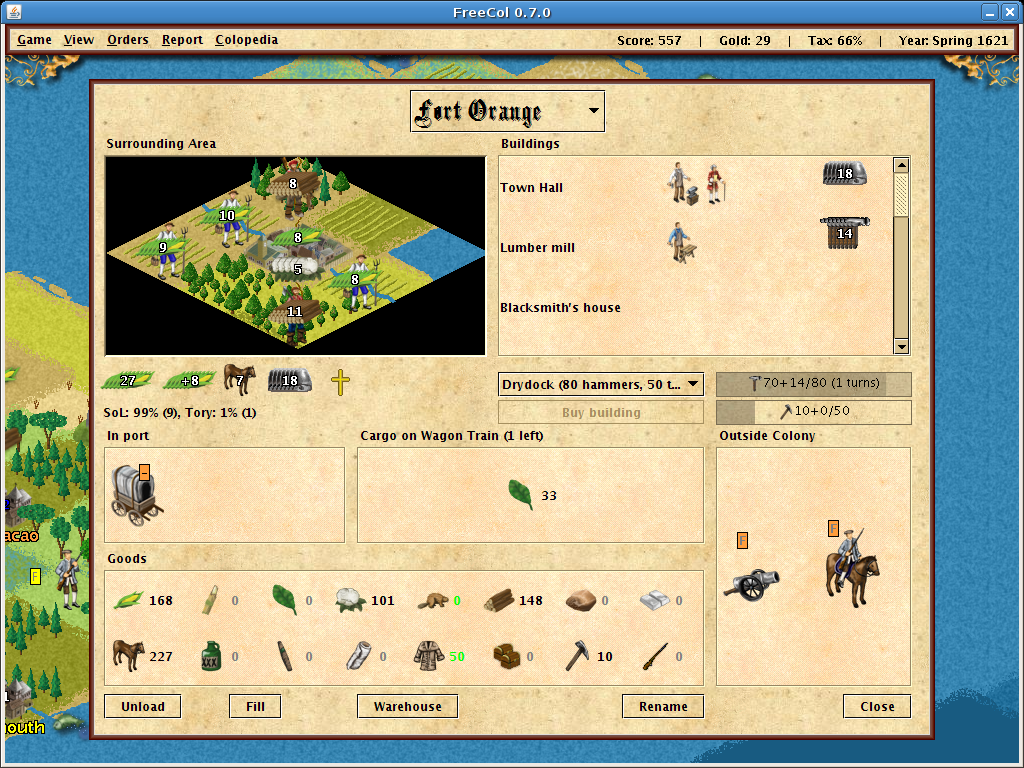
\includegraphics[scale=0.35]{images/colony_panel.png}
    \caption{The Colony Panel.\label{colony_panel_fig}}
  \end{center}
\end{figure}

To view a colony's panel, left click on it from the main
screen. From this panel, colonist's cultivation, production, and other
tasks can be assigned:

\begin{itemize}
\item Cultivation: Drop the unit onto the appropriate plot of land in
  the colony. You can change what a colonist cultivate by right
  clicking on it. Note that your colonists can not go fishing on ocean
  tiles before they have built a dock.
\item Production: Drop the unit onto the relevant �Buildings�.
\item Depart colony: Drop the unit onto the colony's gate.
\item Embark on a ship: If there is a ship in port, you can embark
  your colonist on it by dropping it onto the �Cargo� section of the
  colony panel.
\item Build a building: Drop the unit onto the carpenter's house and
  select the building you want from the building menu.
\end{itemize}

You can also load cargo into a ship's hold by dropping the goods onto
the ship or the specific hold within the ship. Use the shift key while
dropping it if you want to load only a portion of the goods.

\hypertarget{Colonies}{\section{Colonies}}

\hypertarget{Picking a suitable site}{\subsection{Picking a suitable site}}

Your colonies are your most important assets in the new world.
Therefore, it is very important to build them in the right
place. There are several aspects to consider:

\hypertarget{The colony tile}{\subsubsection{The colony tile}}

Some terrain types are more suitable for establishing a colony than
others. Colonies can not be built on arctic tiles, nor on
mountains. Hills and deserts are less suitable than other tiles
because they produce less food, which is very important in the long
run. Tiles with forest generally produce less food than tiles without,
but pioneers are able to cut down the forest and plow the tile, which
will increase food production. The presence of a river will also
increase food production.

\hypertarget{The adjacent tiles}{\subsubsection{The adjacent tiles}}

In the early stages of the game, you will need to generate cash by
selling products from the New World in your Home Port. Thus, many of
your early colonies should probably be situated next to bonus tiles,
which greatly increase production. Rivers also increase production,
though not as much as a bonus resource. On the other hand, they
increase the production of many different kinds of goods, unlike a
bonus resource.

In order to improve your colony, you will have to construct various
buildings. This will require large amounts of lumber. For this reason,
you should make sure that at least one tile adjacent to your colony
site can produce sufficient amounts of lumber. You will also need
tools to construct advanced buildings. Therefore, it is an advantage
if the colony can also produce ore, which can be refined to produce
tools. However, ore is not as important as lumber.

Some of the tiles may be owned by other European powers, or claimed by
Indians. Building a colony too close to other settlements is not a
good idea, unless you plan to conquer or destroy these settlements.
Keeping your own colonies close together is a good strategy, however,
as long as you avoid sharing tiles between several colonies as far as
possible.

\hypertarget{No Reforestation}{\subsubsection{No Reforestation}}

You can order your pioneers to cut down forests by plowing a tile.
This will increase the food produced on these tiles, and the lumber
will be delivered to your colonies. However, you can not plant new
forests later. Once cleared, a tile will never produce lumber again.

\hypertarget{Colony Buildings}{\subsection{Colony Buildings}}

A newly established colony already includes several buildings, namely
a town hall, a carpenter's house, a blacksmith's house, a
tobacconist's house, a weaver's house, a distiller's house, a fur
trader's house, and a warehouse. You can improve your colonies by
upgrading all of these buildings except the town hall, and by
constructing various new buildings. However, many buildings can only
be constructed in colonies of a certain size, or after certain
\hyperlink{Founding Fathers}{Founding Fathers} have joined the
\hyperlink{Continental Congress}{Continental Congress}.

The craftsmen's houses can be upgraded to workshops, which produce
more manufactured goods. After \hyperlink{Adam Smith}{Adam Smith} has
joined the \hyperlink{Continental Congress}{Continental Congress},
workshops can be upgraded to factories, which produce one and a half
units of manufactured goods from each unit of raw material. While the
town hall itself can not be upgraded, the production of
\hyperlink{Liberty Bells}{Liberty Bells} can be boosted by
constructing a printing press and then a newspaper.

All in all, there are sixteen different buildings, eight of which are
immediately present in a newly established colony:

\begin{itemize}
\item The \hypertarget{Town Hall}{\textbf{Town Hall}}, which can not
  be upgraded, provides workplaces for up to three colonists producing
  \textbf{Liberty Bells}. Its effect can be increased by building a
  \hyperlink{Printing Press}{Printing Press} and a
  \hyperlink{Newspaper}{Newspaper}.

\item The \hypertarget{Carpenter's House}{\textbf{Carpenter's House}},
  which can be upgraded to a \textbf{Lumber Mill} once the colony's
  population reaches 3, is used to convert \hyperlink{Lumber}{Lumber}
  to \hyperlink{Hammers}{Hammers}. Hammers are required to construct
  or upgrade all kinds of buildings.

\item The \hypertarget{Blacksmith's House}{\textbf{Blacksmith's
  House}}, which can be upgraded to a \hypertarget{Blacksmith's
  Workshop}{\textbf{Blacksmith's Workshop}}, is used to convert
  \hyperlink{Ore}{Ore} to \hyperlink{Tools}{Tools}. Tools are required
  to construct certain kinds of buildings and to upgrade all kinds of
  buildings. Tools are also used by \hyperlink{Pioneers}{Pioneers} and
  to produce \hyperlink{Muskets}{Muskets}. Once the population of the
  colony has reached 8, the Blacksmith's Workshop can be replaced by
  \hypertarget{Iron Works}{\textbf{Iron Works}}, provided that
  \hyperlink{Adam Smith}{Adam Smith} has joined the
  \hyperlink{Continental Congress}{Continental Congress}.

\item The \hypertarget{Tobacconist's House}{\textbf{Tobacconist's
  House}}, which can be upgraded to a \hypertarget{Tobacconist's
  Shop}{\textbf{Tobacconist's Shop}}, is used to produce
  \hyperlink{Cigars}{Cigars} from \hyperlink{Tobacco}{Tobacco}.  Once
  the colony's population has reached 8, it can be further upgraded to
  a \hypertarget{Cigar Factory}{\textbf{Cigar Factory}}, provided that
  \hyperlink{Adam Smith}{Adam Smith} has joined the
  \hyperlink{Continental Congress}{Continental Congress}.

\item The \hypertarget{Weaver's House}{\textbf{Weaver's House}},
  which can be upgraded to a \hypertarget{Weaver's
  Shop}{\textbf{Weaver's Shop}}, is used to turn
  \hyperlink{Cotton}{Cotton} into \hyperlink{Cloth}{Cloth}. It can be
  upgraded to a \hypertarget{Textile Mill}{\textbf{Textile Mill}} as
  soon as the population of the colony is at least 8 and
  \hyperlink{Adam Smith}{Adam Smith} has joined the
  \hyperlink{Continental Congress}{Continental Congress}.

\item The \hypertarget{Distiller's House}{\textbf{Distiller's
  House}}, which can be upgraded to a \hypertarget{Rum
  Distillery}{\textbf{Rum Distillery}}, is used to produce
  \hyperlink{Rum}{Rum} from \hyperlink{Sugar}{Sugar}. Once
  \hyperlink{Adam Smith}{Adam Smith} has joined the
  \hyperlink{Continental Congress}{Continental Congress} and the
  colony's population is at least 8, the rum distillery can be
  replaced by a \hypertarget{Rum Factory}{\textbf{Rum Factory}}.

\item The \hypertarget{Fur Trader's House}{\textbf{Fur Trader's
  House}}, which can be upgraded to a \hypertarget{Fur Trader's
  Post}{\textbf{Fur Trader's Post}}, is used to produce
  \hyperlink{Coats}{Coats} from \hyperlink{Fur}{Fur}. Once the
  colony's population has reached 6, it can be further upgraded to a
  \hypertarget{Fur Factory}{\textbf{Fur Factory}}, provided that
  \hyperlink{Adam Smith}{Adam Smith} has joined the
  \hyperlink{Continental Congress}{Continental Congress}.

\item The \hypertarget{Warehouse}{\textbf{Warehouse}} stores all kinds
  of goods. Its initial capacity is 100 units of each kind of goods,
  but it can be upgraded to 200 and finally 300 units.
\end{itemize}

The following eight buildings are not available for free and have to
be constructed later:

\begin{itemize}
\item A colony with a population of at least 4 may build a 
  \hypertarget{Schoolhouse}{\textbf{Schoolhouse}}, which enables some
  master craftsman to teach an unskilled colonist their trade. As soon
  as the population reaches 8, it can be upgraded to a
  \hypertarget{College}{\textbf{College}}, in which additional trades
  can be taught by two colonists. Once the population reaches 10, the
  college can be replaced by a
  \hypertarget{University}{\textbf{University}}, at which all trades
  can be taught by three colonists. See \hyperlink{Skills and
  Education}{Skills and Education} for details.

\item The \hypertarget{Armory}{\textbf{Armory}} is used to produce
  \hyperlink{Muskets}{Muskets} from \hyperlink{Tools}{Tools}. As soon
  as the population reaches 8, the armory can be upgraded to a
  \hypertarget{Magazine}{\textbf{Magazine}} and then to an
  \hypertarget{Arsenal}{\textbf{Arsenal}}, provided that
  \hyperlink{Adam Smith}{Adam Smith} has joined the
  \hyperlink{Continental Congress}{Continental Congress}.

\item A colony with a population of 3 or more may build a
  \hypertarget{Church}{\textbf{Church}}, which can be upgraded to a
  \hypertarget{Cathedral}{\textbf{Cathedral}} as soon as the
  population reaches 8. The religious freedom of the New World
  (symbolized by \hyperlink{Crosses}{Crosses}) causes increased
  emigration from Europe.

\item The \hypertarget{Stockade}{\textbf{Stockade}}, which can be
  constructed as soon as the colony's population reaches 3, protects
  the colonists from attacks. Note that a colony with a stockade can
  not be abandoned, it can only be burned to the ground by
  natives. The stockade can be upgraded to a
  \hypertarget{Fort}{\textbf{Fort}}, which provides better protection
  and bombards \hyperlink{Privateers}{Privateers} and enemy naval
  units on adjacent ocean tiles. The fort can be replaced by a
  \hypertarget{Fortress}{\textbf{Fortress}} as soon as the population
  reaches 8.

\item The \hypertarget{Stables}{\textbf{Stables}} increase the
  production of \hyperlink{Horses}{Horses}.

\item The \hypertarget{Dock}{\textbf{Dock}} allows colonists to 
  produce \hyperlink{Fish}{Fish} on ocean tiles adjacent to the
  colony. As soon as the population is at least 4, it can be upgraded
  to a \hypertarget{Drydock}{\textbf{Drydock}}, which allows the
  colony to repair damaged ships. When the colony's population reaches
  8, it can be further upgraded to a
  \hypertarget{Shipyard}{\textbf{Shipyard}}, which enables the colony
  to build new ships.

\item The \hypertarget{Printing Press}{\textbf{Printing Press}}, 
  which can be upgraded to a
  \hypertarget{Newspaper}{\textbf{Newspaper}} as soon as the
  population reaches 4, increases the colony's production of
  \hyperlink{Liberty Bells}{Liberty Bells}.

\item The \hypertarget{Custom House}{\textbf{Custom House}}, which can
  be built as soon as \hyperlink{Peter Stuyvesant}{Peter Stuyvesant}
  has joined the \hyperlink{Continental Congress}{Continental
  Congress}, allows the colony to export goods to Europe directly
  without the help of ships. Optionally, it may also ignore
  \hyperlink{Boycotts}{Boycotts}.

\end{itemize}



\hypertarget{Skills and Education}{\section{Skills and Education}}

In FreeCol, your colonists come from all walks of life. Some are
unskilled \hypertarget{Petty Criminals}{\textbf{Petty Criminals}}, who
are deported to the colonies. Others are \hypertarget{Indentured
Servants}{\textbf{Indentured Servants}}, or \hypertarget{Free
Colonists}{\textbf{Free Colonists}} with moderate skills. Still others
are masters of their craft, experts at their trade or profession, who
were educated at the Royal College in Europe. If you have enough gold,
you can recruit units directly from the Royal College.

Not all skills, however, can be learned in Europe. The cultivation of
\hyperlink{Sugar}{Sugar}, \hyperlink{Cotton}{Cotton} and
\hyperlink{Tobacco}{Tobacco} is unknown in Europe. Thus,
\hypertarget{Master Sugar Planters}{\textbf{Master Sugar
Planters}}, \hypertarget{Master Sugar Planters}{\textbf{Master Cotton
Planters}}, \hypertarget{Master Sugar Planters}{\textbf{Master Tobacco
Planters}}, as well \hypertarget{Master Fur Trappers}{\textbf{Master
Fur Trappers}}, can not be recruited in Europe.

At the beginning of the game, these skills can only be learned at
Indian Settlements. As soon as you construct a
\hyperlink{Schoolhouse}{Schoolhouse}, however, you can order your
master craftsmen to teach other free colonists their skills. Petty
criminals and indentured servants can not become master craftsmen.
However, a petty criminal may become an indentured servant, and an
indentured servant may become a free colonist through education.

Indian units are more productive than free colonists when working
outside of the colony, and less productive when working inside a
building. Indian units can not become free colonists through
education, but all Indian units become free colonists as soon as
\hyperlink{Bartolome de las Casas}{Bartolome de las Casas} joins the
\hyperlink{Continental Congress}{Continental Congress}.



\hypertarget{Copyright Notice}{\section{Copyright Notice}}
Copyright � 2006
\href{http://freecol.sourceforge.net/index.php?section=8}{The FreeCol
Team}.

This manual is free software; you may redistribute it and/or modify it
under the terms of the GNU General Public License as published by the
Free Software Foundation; either version 2, or (at your option) any
later version.

This is distributed in the hope that it will be useful, but without
any warranty; without even the implied warranty of merchantability or
fitness for a particular purpose. See the GNU General Public License
for more details.

A copy of the GNU General Public License is available on the World
Wide Web at \href{http://www.gnu.org/copyleft/gpl.html}{the GNU
General Public Licence}. You can also obtain it by writing to the Free
Software Foundation, Inc., 59 Temple Place - Suite 330, Boston, MA
02111-1307, USA.

\end{document}
